\begin{frame}{形状作成}
  %
   \begin{columns}[t]
    \begin{column}{0.65\textwidth}
      \\
      今回はgmshの形状作成機能を使って、回転体で\\
      作ります \\
      ただし、今回の場合、形状に問題発生(後述) \\
      \vspace{5mm}
      後ほどgmshのセーブファイルを公開しますので、\\
      詳細の説明は省くものの、後で作成詳細をなぞる\\
      ことが可能です
    \end{column}
    \begin{column}{0.35\textwidth}
      \begin{figure}[htbp]
        \begin{center}
          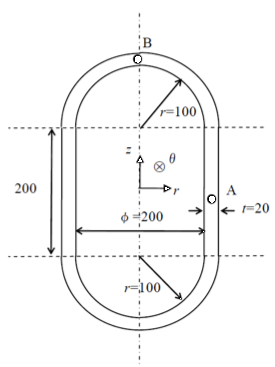
\includegraphics[keepaspectratio,scale=2.2]{images/example-probrem.png}
            \caption{本日の例題(圧力容器・再掲)}
        \end{center}
      \end{figure}
    \end{column}
  \end{columns}
\end{frame}
